\documentclass[aspectratio=169,10pt]{beamer}

\usepackage[T1]{fontenc}
\usepackage[utf8]{inputenc}
\usepackage[spanish,es-minimal,es-noshorthands]{babel}
\usepackage{amsmath,amssymb,bm}
\usepackage{booktabs}
\usepackage{listings}
\usepackage{tikz}
\usetikzlibrary{positioning,arrows.meta,calc,fit,shapes.misc,decorations.pathreplacing}

\usetheme[progressbar=frametitle,numbering=fraction,sectionpage=progressbar]{metropolis}
\definecolor{azul}{HTML}{2C4A8C}
\definecolor{rojo}{HTML}{C8412C}
\definecolor{naranja}{HTML}{F4A261}
\definecolor{celeste}{HTML}{CFE6FB}
\definecolor{verde}{HTML}{2E8B57}
\definecolor{fondo}{HTML}{1F2F4A}
\setbeamercolor{frametitle}{bg=fondo,fg=white}
\setbeamercolor{progress bar}{fg=rojo,bg=celeste}
\setbeamercolor{alerted text}{fg=rojo}
\setbeamercolor{block title}{bg=celeste!70,fg=fondo}
\setbeamercolor{block body}{bg=celeste!25}
\setbeamercolor{block title alerted}{bg=rojo!85,fg=white}
\setbeamercolor{block body alerted}{bg=rojo!8}
\setbeamercolor{block title example}{bg=verde!80,fg=white}
\setbeamercolor{block body example}{bg=verde!8}
\metroset{block=fill}

\lstset{basicstyle=\ttfamily\scriptsize,keywordstyle=\color{azul}\bfseries,commentstyle=\color{verde},
        stringstyle=\color{rojo},columns=fullflexible,keepspaces=true,showstringspaces=false,
        language=Python,frame=single,rulecolor=\color{celeste},backgroundcolor=\color{celeste!15},
        literate={á}{{\'a}}1 {é}{{\'e}}1 {í}{{\'i}}1 {ó}{{\'o}}1 {ú}{{\'u}}1 {ñ}{{\~n}}1
                 {χ}{{$\chi$}}1 {ψ}{{$\psi$}}1 {κ}{{$\kappa$}}1 {π}{{$\pi$}}1 {≤}{{$\le$}}1}

\graphicspath{{imagenes_pwe/}{imagenes/}{../results/}}
\IfFileExists{../results/comparison/tables/efficiency_macros.tex}
  {% Generado por scripts/comparison/efficiency.py: cifras de tiempo del anexo y del paper.
\providecommand{\EffAlpha}{2.52}
\providecommand{\EffAlphaShort}{2.5}
\providecommand{\EffProdBeta}{0.96}
\providecommand{\EffTmmRecMin}{0.23}
\providecommand{\EffTmmRecMax}{0.33}
\providecommand{\EffTmmScalar}{44}
\providecommand{\EffTmmMaxM}{20}
\providecommand{\EffTmmMaxLayers}{10\,946}
\providecommand{\EffProdFirst}{0.5}
\providecommand{\EffProdLast}{291}
\providecommand{\EffPweFirstM}{2}
\providecommand{\EffPweFirst}{3.3~ms}
\providecommand{\EffPweLastM}{10}
\providecommand{\EffPweLast}{32.5~s}
\providecommand{\EffPweGrowth}{3.4}
\providecommand{\EffExtrapAM}{12}
\providecommand{\EffExtrapA}{6~min}
\providecommand{\EffExtrapBM}{15}
\providecommand{\EffExtrapB}{3.7~h}
\providecommand{\EffExtrapBMem}{16~GB}
\providecommand{\EffMemEight}{19~MB}
\providecommand{\EffWpM}{5}
\providecommand{\EffWpTmmErr}{3\times10^{-15}}
\providecommand{\EffWpTmmMin}{1.4}
\providecommand{\EffWpTmmMax}{31}
\providecommand{\EffWpErrExp}{3.1}
\providecommand{\EffWpTimeExp}{2.5}
\providecommand{\EffWpTradeExp}{1.3}
\providecommand{\EffWpBestErr}{1\times10^{-6}}
\providecommand{\EffWpBestN}{385}
\providecommand{\EffWpBestTime}{1.2~s}
\providecommand{\EffWpSpeedRatio}{4\times10^{4}}
\providecommand{\EffWpErrRatio}{4\times10^{8}}
\providecommand{\EffWpTargetN}{3\times10^{4}}
\providecommand{\EffWpTargetMem}{68~GB}
\providecommand{\EffWpTargetTime}{23~h}
\providecommand{\EffFigTmmTotal}{0.32~s}
\providecommand{\EffFigPweTotal}{5.3~h}
\providecommand{\EffFigRatioMin}{2\times10^{4}}
\providecommand{\EffFigRatioMax}{4\times10^{5}}
\providecommand{\EffFigWallMin}{45}
\providecommand{\EffFigWallMax}{319}
\providecommand{\EffFigTmmMin}{2.9}
\providecommand{\EffFigTmmMax}{3.4}
\providecommand{\EffBookN}{101}
\providecommand{\EffBookPwe}{116~ms}
\providecommand{\EffBookTmm}{78~ms}
\providecommand{\EffBookGrid}{14~ms}
\providecommand{\EffBookGridPoints}{60\,001}
\providecommand{\EffBookErr}{5\times10^{-6}}
}{}

\newcommand{\nue}{\nu_e}
\newcommand{\num}{\nu_m}
\newcommand{\toep}[1]{[\![#1]\!]}
\newcommand{\kt}{\tilde k}
\newcommand{\figfull}[1]{\includegraphics[width=\linewidth,height=0.78\textheight,keepaspectratio]{#1}}

\title{El método de ondas planas (PWE) para superredes de Fibonacci}
\subtitle{Del libro de Sukhoivanov y Guryev al metamaterial de Drude}
\author{Emanuel Orozco Gallego}
\institute{Análisis Numérico}
\date{}

\begin{document}

\maketitle

\begin{frame}{Contenido}
  \begin{columns}[T]
    \begin{column}{0.48\textwidth}
      \tableofcontents[sections={1-4},hideallsubsections]
    \end{column}
    \begin{column}{0.48\textwidth}
      \tableofcontents[sections={5-8},hideallsubsections]
    \end{column}
  \end{columns}
\end{frame}

% =====================================================================
\section{Motivación}
% =====================================================================

\begin{frame}{El problema en una imagen}
  \begin{columns}[c]
    \begin{column}{0.55\textwidth}
      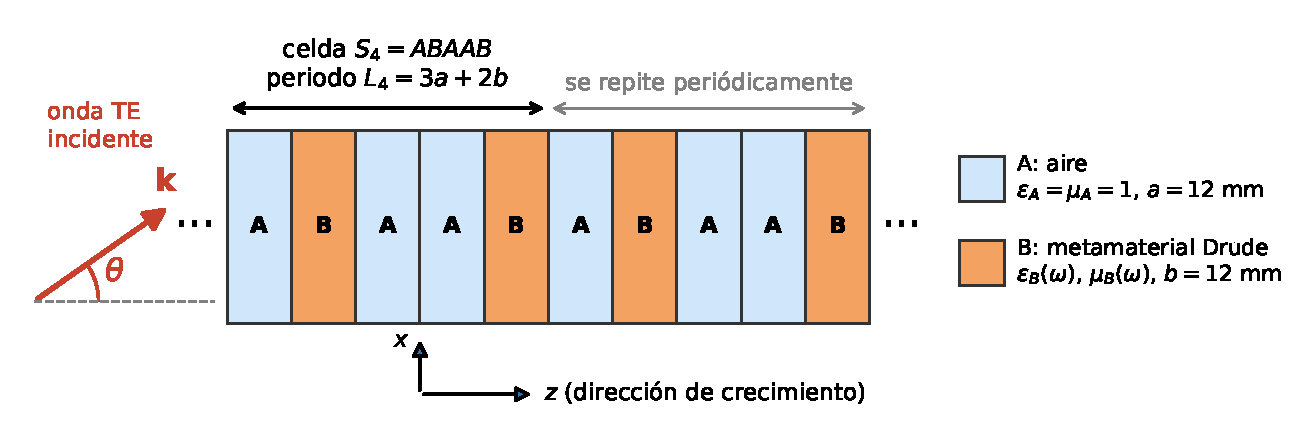
\includegraphics[width=\linewidth]{superred_geometria.pdf}
    \end{column}
    \begin{column}{0.43\textwidth}
      \small
      \begin{itemize}
        \item Superred cuya celda es la palabra de Fibonacci $S_m$: capas de aire (A) y de metamaterial (B).
        \item B tiene respuesta de Drude:
          \[\varepsilon_B=1-\frac{\omega_e^2}{\omega^2},\qquad \mu_B=1-\frac{\omega_m^2}{\omega^2}.\]
        \item La pregunta del paper: ¿para qué frecuencias hay \textbf{bandas} (la onda se propaga) y
          para cuáles hay \textbf{gaps}?
        \item Todo se resume en la semitraza
          \[R_m=\cos(kL_m):\quad |R_m|\le1 \Rightarrow \text{banda}.\]
      \end{itemize}
    \end{column}
  \end{columns}
\end{frame}

\begin{frame}{¿Por qué un segundo método si ya tenemos la TMM?}
  \begin{columns}[T]
    \begin{column}{0.48\textwidth}
      \begin{block}{Matriz de transferencia (TMM)}
        \small
        \begin{itemize}
          \item Multiplica matrices $2\times2$ capa por capa.
          \item Exacta para medios estratificados.
          \item Es el método de producción del proyecto.
        \end{itemize}
      \end{block}
      \begin{block}{Ondas planas (PWE)}
        \small
        \begin{itemize}
          \item Desarrolla campos y materiales en series de Fourier.
          \item Convierte la ecuación de onda en un \textbf{problema de autovalores}.
          \item Es el método estándar de los cristales fotónicos 2D y 3D.
        \end{itemize}
      \end{block}
    \end{column}
    \begin{column}{0.48\textwidth}
      \begin{exampleblock}{Para qué sirve aquí}
        \small
        \begin{enumerate}
          \item \textbf{Verificación independiente}: parte de otra formulación (espacio recíproco), así que
            si coincide con la TMM, ambos resultados se refuerzan.
          \item \textbf{Base para 2D}, donde la TMM ya no se aplica.
          \item \textbf{Aprendizaje}: el metamaterial de Drude rompe la receta del libro y obliga a
            entender el método a fondo.
        \end{enumerate}
      \end{exampleblock}
      \vspace{0.2em}
      \footnotesize Fuente del método: I.\,A.\ Sukhoivanov e I.\,V.\ Guryev, \textit{Photonic Crystals},
      cap.~4, y su cuaderno \texttt{PWE-1d.ipynb}.
    \end{column}
  \end{columns}
\end{frame}

\begin{frame}{Hoja de ruta}
  \centering
  \begin{tikzpicture}[
      caja/.style={rounded corners=4pt,draw=fondo,fill=celeste!55,line width=0.8pt,
                   minimum width=3.3cm,minimum height=1.3cm,align=center,font=\small},
      flecha/.style={-{Stealth[length=3mm]},line width=1.2pt,fondo},
      node distance=0.8cm and 0.8cm]
    \node[caja] (a) {\textbf{1. Conceptos}\\Bloch, Fourier,\\red recíproca};
    \node[caja,right=of a] (b) {\textbf{2. PWE del libro}\\problema de\\autovalores $\omega(k)$};
    \node[caja,right=of b] (c) {\textbf{3. Validación}\\cristal del libro\\$\varepsilon_1=1$, $\varepsilon_2=9$};
    \node[caja,below=of c,fill=rojo!25] (d) {\textbf{4. El reto}\\Drude: $\omega(k)$ falla};
    \node[caja,left=of d,fill=verde!25] (e) {\textbf{5. La solución}\\$k(\omega)$ + regla\\inversa de Li};
    \node[caja,left=of e,fill=naranja!45] (f) {\textbf{6. Código y}\\\textbf{resultados}\\Figs.~1--6 del paper};
    \draw[flecha] (a) -- (b);
    \draw[flecha] (b) -- (c);
    \draw[flecha] (c) -- (d);
    \draw[flecha] (d) -- (e);
    \draw[flecha] (e) -- (f);
  \end{tikzpicture}
\end{frame}

% =====================================================================
\section{Conceptos necesarios}
% =====================================================================

\begin{frame}{Una sola ecuación para TE y TM}
  \begin{columns}[T]
    \begin{column}{0.55\textwidth}
      \small
      El medio cambia solo en $z$; la onda viaja en el plano $xz$ con componente tangencial
      conservada $q=\frac{\omega}{c}n_A\sin\theta$. La componente transversal $u(z)$ cumple
      \begin{block}{Ecuación de onda estratificada}
        \[\frac{d}{dz}\!\left[\frac{1}{\chi(z)}\frac{du}{dz}\right]
          +\left(\kappa^2\psi(z)-\frac{q^2}{\chi(z)}\right)u=0,\quad \kappa=\frac{\omega}{c}\]
      \end{block}
      \begin{center}
        \begin{tabular}{cccc}
          \toprule
          Polarización & $u$ & $\chi$ (dentro de la derivada) & $\psi$ \\
          \midrule
          TE & $E_y$ & $\mu$ & $\varepsilon$ \\
          TM & $H_y$ & $\varepsilon$ & $\mu$ \\
          \bottomrule
        \end{tabular}
      \end{center}
    \end{column}
    \begin{column}{0.42\textwidth}
      \begin{alertblock}{Qué es continuo en cada interfaz}
        \small
        \begin{itemize}
          \item El campo $u$.
          \item El \textbf{flujo} $D=\dfrac{1}{\chi}\dfrac{du}{dz}$.
        \end{itemize}
        $u'$ y $1/\chi$ saltan por separado; su producto no. Este detalle decidirá cómo se
        discretiza el método (regla de Li).
      \end{alertblock}
      \small En TE (el caso del paper) la función que salta dentro de la derivada es $\mu$, justo la
      que se anula en $\num$.
    \end{column}
  \end{columns}
\end{frame}

\begin{frame}{Cristal periódico y teorema de Bloch}
  \begin{columns}[c]
    \begin{column}{0.60\textwidth}
      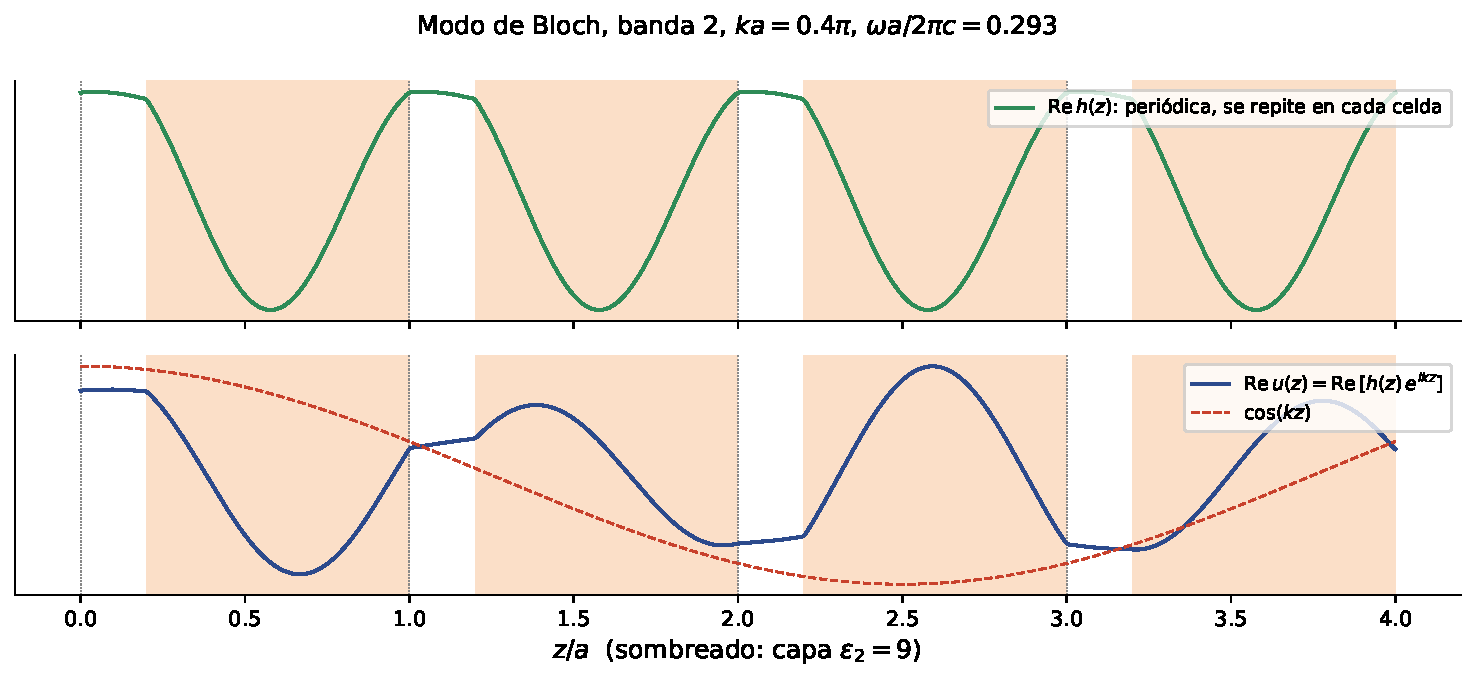
\includegraphics[width=\linewidth]{bloch_onda.pdf}
    \end{column}
    \begin{column}{0.38\textwidth}
      \footnotesize
      Si $\chi$ y $\psi$ se repiten con período $L$, las soluciones son \textbf{ondas de Bloch}:
      \[u(z)=h(z)\,e^{ikz},\qquad h(z+L)=h(z).\]
      \begin{itemize}
        \item $h$: la ``forma'' del modo dentro de una celda.
        \item $e^{ikz}$: una onda plana que avanza de celda en celda.
        \item Al pasar una celda, el campo solo gana la fase $e^{ikL}$. Por eso
          \[\cos(kL)=\tfrac12\operatorname{Tr}T=R.\]
      \end{itemize}
      TMM y PWE calculan la \textbf{misma} cantidad $R$.
    \end{column}
  \end{columns}
\end{frame}

\begin{frame}{Red directa, red recíproca y zona de Brillouin}
  \centering
  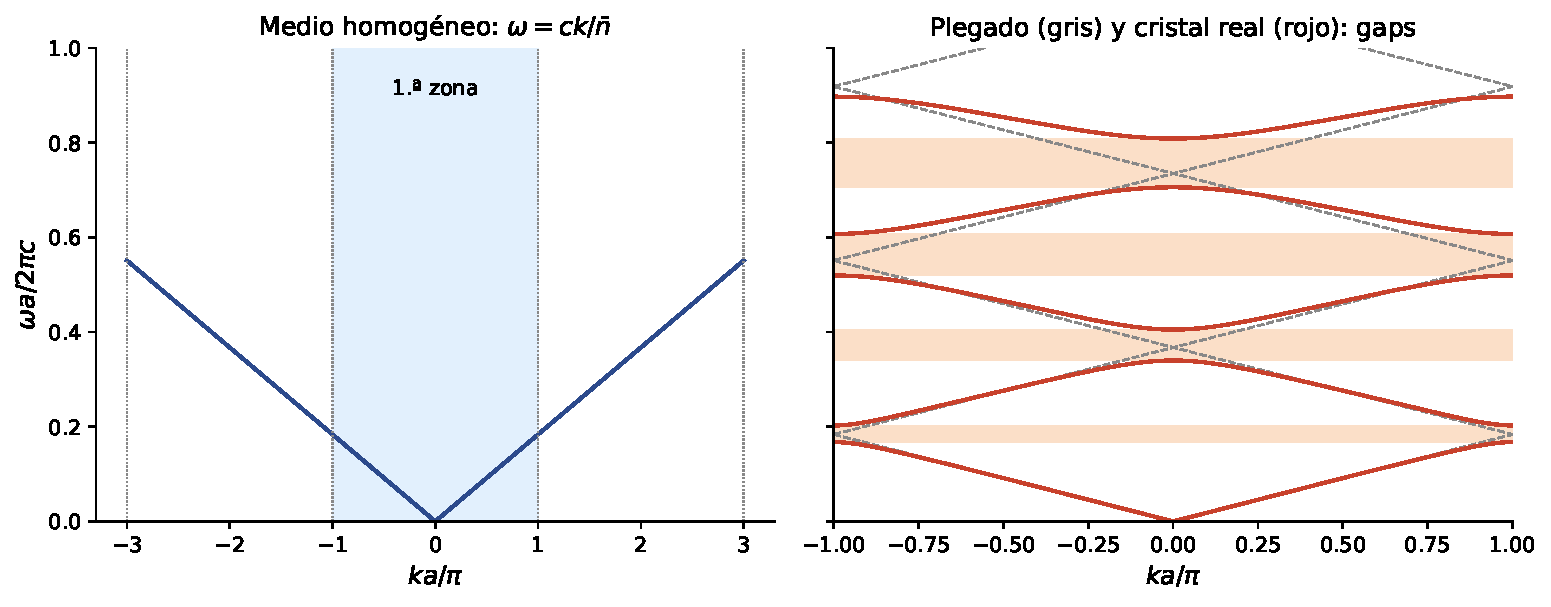
\includegraphics[width=\linewidth,height=0.50\textheight,keepaspectratio]{plegado_bandas.pdf}
  \raggedright\small
  \begin{columns}[T]
    \begin{column}{0.48\textwidth}
      \begin{itemize}
        \item Red directa: $z_\ell=\ell L$. Red recíproca: $G_n=\dfrac{2\pi n}{L}$, con $e^{iG_nL}=1$.
        \item $k$ y $k+G_n$ describen el mismo modo: basta con la \textbf{primera zona}
          $-\pi/L<k\le\pi/L$.
      \end{itemize}
    \end{column}
    \begin{column}{0.48\textwidth}
      \begin{itemize}
        \item La recta de luz se \textbf{pliega} en la zona; donde dos ramas se cruzan, la periodicidad abre un \textbf{gap}.
        \item En la superred $L_m\propto F_m$: la zona se estrecha y hay cada vez más pliegues y subbandas.
      \end{itemize}
    \end{column}
  \end{columns}
\end{frame}

\begin{frame}{Series de Fourier: una función periódica es una suma de ondas planas}
  \centering
  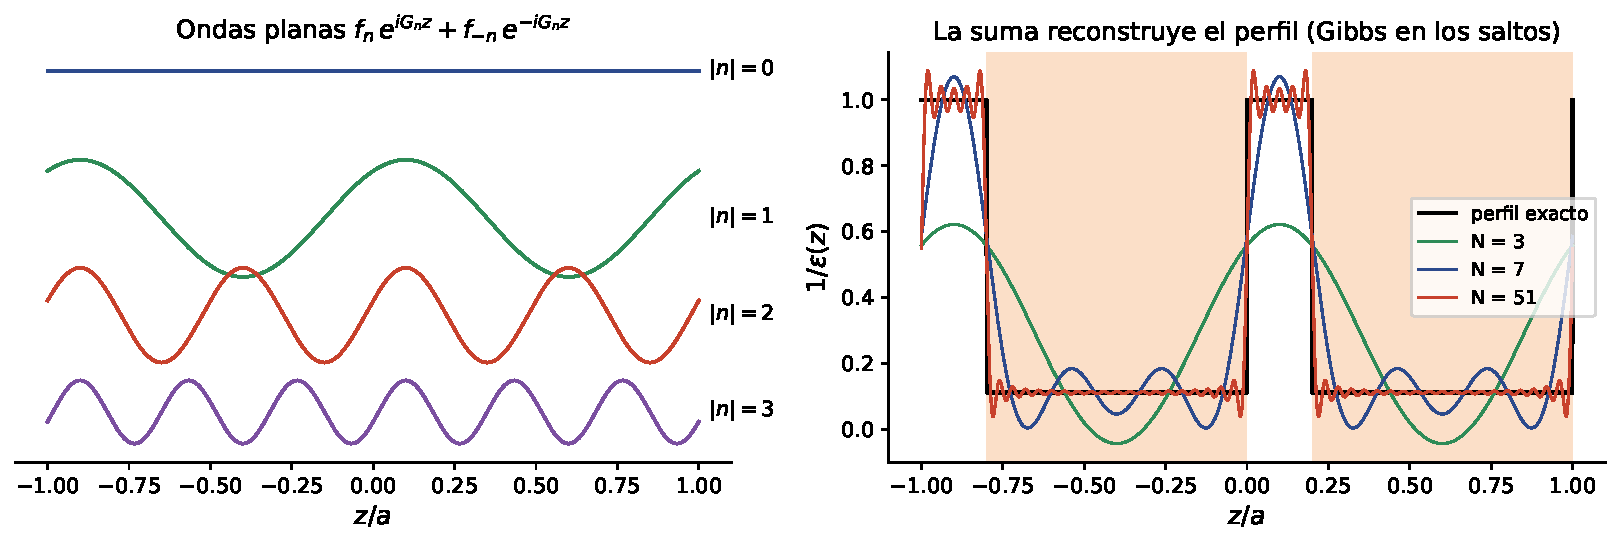
\includegraphics[width=\linewidth,height=0.50\textheight,keepaspectratio]{ondas_planas_suma.pdf}
  \raggedright\small
  \[f(z)=\sum_{n=-\infty}^{\infty} f_n\,e^{iG_nz},\qquad
    f_n=\frac1L\int_0^L f(z)\,e^{-iG_nz}\,dz .\]
  \begin{itemize}
    \item Truncamos a $n=-n_{\max}\dots n_{\max}$: $N=2n_{\max}+1$ ondas planas.
    \item El perfil escalonado converge lento ($f_n\sim1/n$) y con \textbf{Gibbs} (sobreimpulso de $\sim\!9\%$) en cada salto.
  \end{itemize}
\end{frame}

\begin{frame}{Coeficientes de la celda de Fibonacci en forma cerrada}
  \begin{columns}[T]
    \begin{column}{0.48\textwidth}
      \small
      Para un perfil constante por tramos ($f=f_j$ en $[z_j,z_{j+1})$):
      \[f_n=\sum_j f_j\,\frac{i}{G_nL}\left(e^{-iG_nz_{j+1}}-e^{-iG_nz_j}\right),\quad n\ne0.\]
      \begin{itemize}
        \item Con dos capas es la ec.~(4.38) del libro.
        \item Como cada capa es A o B:
          \[f_n=f_A\,(\mathbb 1_A)_n+f_B\,(\mathbb 1_B)_n .\]
        \item Los coeficientes de las indicadoras se calculan \textbf{una vez}; para cada frecuencia
          basta combinar dos vectores, aunque $\mu_B<0$ o dependa de $\omega$.
      \end{itemize}
    \end{column}
    \begin{column}{0.50\textwidth}
      \centering
      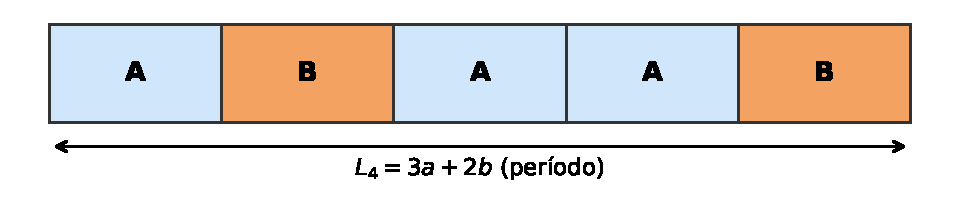
\includegraphics[width=0.75\linewidth]{celda_s4.pdf}\\[0.2em]
      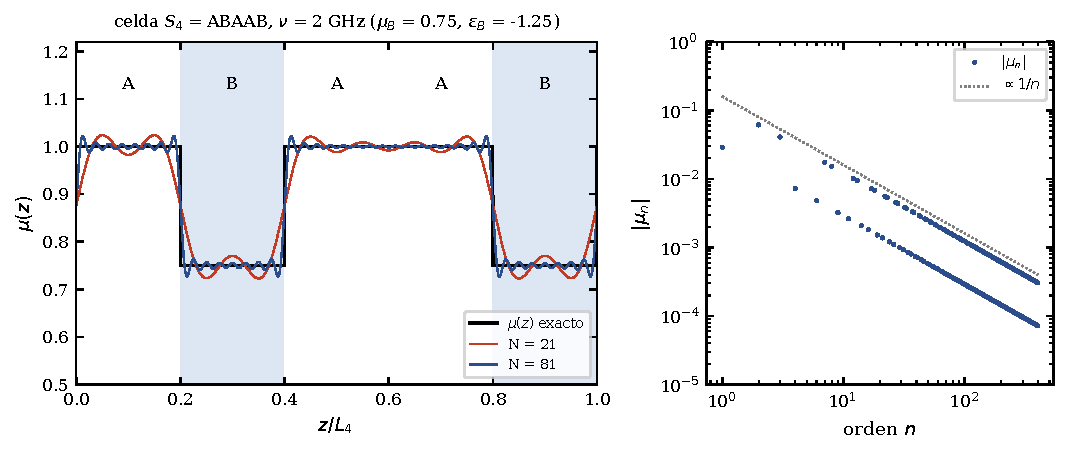
\includegraphics[width=\linewidth,height=0.40\textheight,keepaspectratio]{pwe/cell_fourier/output/cell_fourier.pdf}\\[0.2em]
      \raggedright\footnotesize Perfil $\mu(z)$ de $S_4$ y su síntesis con $N=21$ y $81$; $|\mu_n|$
      decae como $1/n$. Código: \texttt{solvers/pwe/fourier.py}.
    \end{column}
  \end{columns}
\end{frame}

\begin{frame}{Producto de funciones $\Rightarrow$ matriz de Toeplitz}
  \begin{columns}[c]
    \begin{column}{0.60\textwidth}
      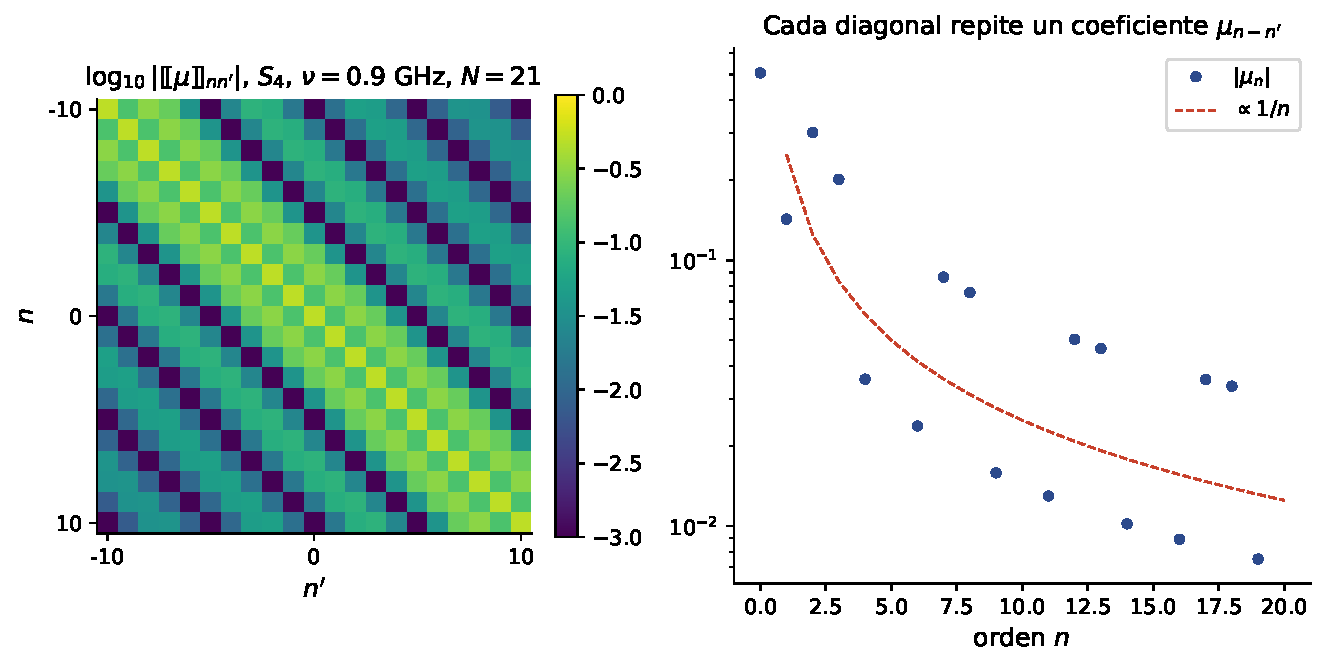
\includegraphics[width=\linewidth]{toeplitz.pdf}
    \end{column}
    \begin{column}{0.38\textwidth}
      \small
      Multiplicar dos funciones periódicas es \textbf{convolucionar} sus coeficientes:
      \[(fu)_n=\sum_{n'}f_{n-n'}\,u_{n'} .\]
      Con $N$ ondas planas eso es una matriz
      \[\toep{f}_{nn'}=f_{n-n'},\]
      constante en cada diagonal (\textbf{Toeplitz}). Necesita los coeficientes hasta $|n|=2n_{\max}$.
      \vspace{0.3em}

      En código: \texttt{CellFourier.toeplitz(f\_A, f\_B)}.
    \end{column}
  \end{columns}
\end{frame}

\begin{frame}{La ecuación maestra: de una EDO a un problema de autovalores}
  \small
  Sustituimos $u(z)=\sum_n u_n\,e^{i(k+G_n)z}$ y los perfiles en Fourier; proyectando sobre cada onda plana:
  \begin{block}{Ecuación maestra (ec.~4.25 del libro, generalizada)}
    \[K\,P\,K\,\mathbf u+q^2\,\toep{1/\chi}\,\mathbf u=\kappa^2\,\toep{\psi}\,\mathbf u,
      \qquad K=\mathrm{diag}(k+G_n)\]
  \end{block}
  \begin{columns}[T]
    \begin{column}{0.48\textwidth}
      \begin{itemize}
        \item $\mathbf u=(u_{-n_{\max}},\dots,u_{n_{\max}})$: coeficientes del modo.
        \item $P$: matriz de $1/\chi$ dentro del flujo (su elección es la \textbf{regla de factorización}).
        \item En el libro (TM, $\mu=1$, $q=0$): $P=\toep{1/\varepsilon}$ y $\psi=1$.
      \end{itemize}
    \end{column}
    \begin{column}{0.48\textwidth}
      \begin{exampleblock}{Medios sin pérdidas ni dispersión}
        $A=KPK+q^2\toep{1/\chi}$ y $B=\toep{\psi}$ son \textbf{hermíticas}, $B>0$:
        \[A\mathbf u=\lambda B\mathbf u,\qquad \lambda=\kappa^2\ge0 .\]
        Se resuelve con \texttt{scipy.linalg.eigh}: para cada $k$ salen $N$ frecuencias.
      \end{exampleblock}
    \end{column}
  \end{columns}
\end{frame}

\begin{frame}{El algoritmo del libro (sección 4.11)}
  \begin{columns}[T]
    \begin{column}{0.50\textwidth}
      \begin{enumerate}
        \item Coeficientes de Fourier del perfil hasta $|n|\le2n_{\max}$.
        \item Recorrer $k$ en la primera zona, $-\pi/L\dots\pi/L$.
        \item Para cada $k$: armar $A$ y $B$ con $N=2n_{\max}+1$ ondas planas.
        \item Autovalores $\lambda$ $\Rightarrow$ $\omega=c\sqrt{\lambda}$.
        \item Dibujar $\omega L/2\pi c$ frente a $k$.
      \end{enumerate}
      \vspace{0.4em}
      \small Es la forma $\boldsymbol{\omega(k)}$: se fija $k$ y se buscan las frecuencias.
      Implementación: \texttt{solvers/pwe/eigenfrequency.py}, \texttt{nondispersive\_bands}.
    \end{column}
    \begin{column}{0.48\textwidth}
      \begin{alertblock}{Truncamiento en la superred}
        \small
        La celda $S_m$ tiene $F_m$ capas, es decir, $F_m$ saltos. Para mantener la misma resolución por capa:
        \[n_{\max}=h\,F_m,\qquad N=2hF_m+1,\]
        con $h$ = armónicos por capa (8 o 16 en este trabajo).
      \end{alertblock}
      \footnotesize
      \begin{center}
        \begin{tabular}{cccc}
          \toprule
          $m$ & capas $F_m$ & $N$ ($h=8$) & $N$ ($h=16$) \\
          \midrule
          3 & 3 & 49 & 97 \\
          4 & 5 & 81 & 161 \\
          5 & 8 & 129 & 257 \\
          6 & 13 & 209 & 417 \\
          \bottomrule
        \end{tabular}
      \end{center}
    \end{column}
  \end{columns}
\end{frame}

% =====================================================================
\section{Validación con el cristal del libro}
% =====================================================================

\begin{frame}{Estructura de bandas: bicapa $\varepsilon_1=1$ / $\varepsilon_2=9$}
  \begin{columns}[c]
    \begin{column}{0.50\textwidth}
      \figfull{pwe/book_benchmark/output/band_structure.pdf}
    \end{column}
    \begin{column}{0.48\textwidth}
      \small
      Parámetros del cuaderno: $l_1=0.2a$, $l_2=0.8a$, $N=101$. Referencia exacta: la TMM de la bicapa.
      \begin{itemize}
        \item Cuadrados: PWE con la regla del libro (Laurent, $P=\toep{1/\varepsilon}$).
        \item Círculos: PWE con la \textbf{regla inversa} ($P=\toep{\varepsilon}^{-1}$).
      \end{itemize}
      \begin{exampleblock}{Residuo máximo $|\cos ka-R_{\rm TMM}(\omega_{\rm PWE})|$}
        Laurent: $0.157$\qquad Inversa: $1.6\times10^{-4}$\\
        con las mismas 101 ondas planas.
      \end{exampleblock}
    \end{column}
  \end{columns}
\end{frame}

\begin{frame}{Convergencia: la regla de factorización lo cambia todo}
  \begin{columns}[c]
    \begin{column}{0.46\textwidth}
      \figfull{pwe/convergence/output/book_convergence.pdf}
    \end{column}
    \begin{column}{0.52\textwidth}
      \small
      Error relativo máximo de las cuatro primeras bandas frente a la TMM, según el número de ondas planas $N$:
      \begin{itemize}
        \item Laurent (libro): error $\propto N^{-1}$.
        \item Inversa (Li): error $\propto N^{-3}$.
      \end{itemize}
      \begin{alertblock}{Lección}
        Para el mismo error, la regla inversa necesita órdenes de magnitud menos ondas planas.
        Con el metamaterial de Drude la diferencia será aún mayor.
      \end{alertblock}
    \end{column}
  \end{columns}
\end{frame}

\begin{frame}{Perfil de campo y bandas fuera del eje}
  \begin{columns}[T]
    \begin{column}{0.45\textwidth}
      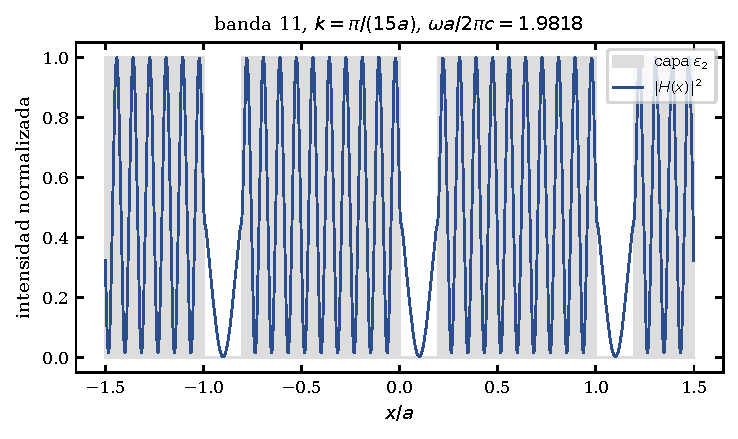
\includegraphics[width=\linewidth]{pwe/book_benchmark/output/field_profile.pdf}\\[0.2em]
      \footnotesize Con los autovectores $u_n$ se reconstruye $H(x)=\sum u_n e^{i(k+G_n)x}$: el campo oscila
      más rápido en la capa de índice alto.
    \end{column}
    \begin{column}{0.53\textwidth}
      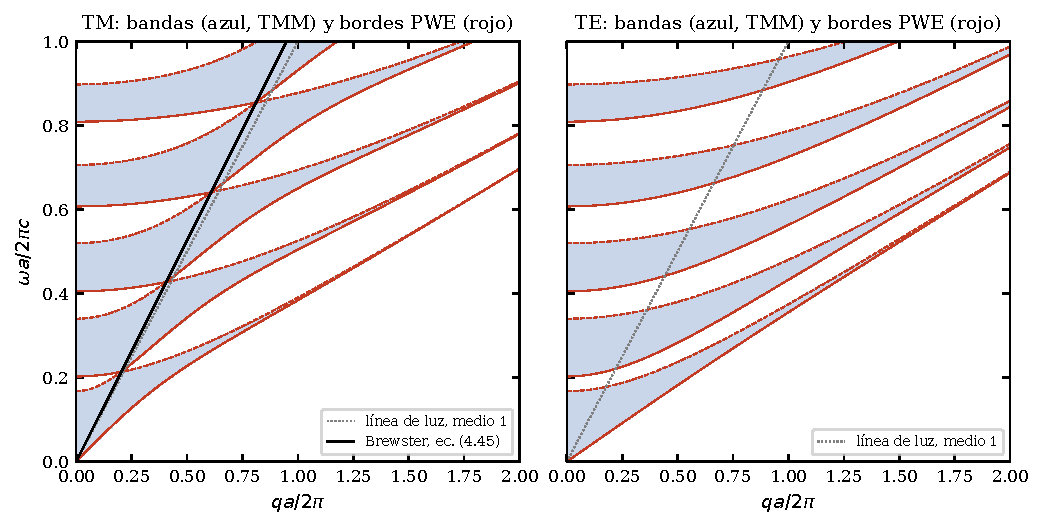
\includegraphics[width=\linewidth]{pwe/book_benchmark/output/off_axis_projected_bands.pdf}\\[0.2em]
      \footnotesize Con $q\ne0$ aparece el término $q^2\toep{1/\chi}$. Fondo: regiones permitidas de la TMM;
      líneas rojas: bordes del PWE. En TM los gaps se cierran sobre la recta de \textbf{Brewster}
      $q_B=\frac{\omega}{c}\frac{n_1n_2}{\sqrt{n_1^2+n_2^2}}$, como indica el libro.
    \end{column}
  \end{columns}
\end{frame}

% =====================================================================
\section{El reto: el metamaterial de Drude}
% =====================================================================

\begin{frame}{Por qué la receta del libro no sirve con Drude}
  \begin{columns}[T]
    \begin{column}{0.50\textwidth}
      \small
      En la superred, $\varepsilon_B(\omega)$ y $\mu_B(\omega)$ \textbf{dependen de la frecuencia}. La ecuación maestra
      \[K P(\omega) K\mathbf u + q^2\toep{1/\chi(\omega)}\mathbf u=\kappa^2\toep{\psi(\omega)}\mathbf u\]
      ya no es lineal en $\lambda=\kappa^2$. Multiplicando por $D(\lambda)=\lambda-\lambda_m$ queda un
      \textbf{problema cuadrático de autovalores} (QEP):
      \[\left[\lambda^2M_2+\lambda M_1+M_0\right]\mathbf u=0,\]
      que se linealiza con una matriz compañera de tamaño $2N$.
    \end{column}
    \begin{column}{0.48\textwidth}
      \begin{alertblock}{Dos problemas}
        \small
        \begin{enumerate}
          \item El término $K\toep{p_0}K$ contiene $D/\mu$, una función escalonada que se anula en las
            capas B: la regla de Laurent no converge.
          \item Cerca de $\mu_B=0$ el operador tiene un \textbf{espectro esencial} en $\num$ (infinitos
            modos localizados), que la discretización imita con una nube de autovalores.
        \end{enumerate}
      \end{alertblock}
      \small Implementado para demostrarlo: \texttt{drude\_qep\_frequencies\_ghz}.
    \end{column}
  \end{columns}
\end{frame}

\begin{frame}{Contaminación espectral}
  \begin{columns}[c]
    \begin{column}{0.58\textwidth}
      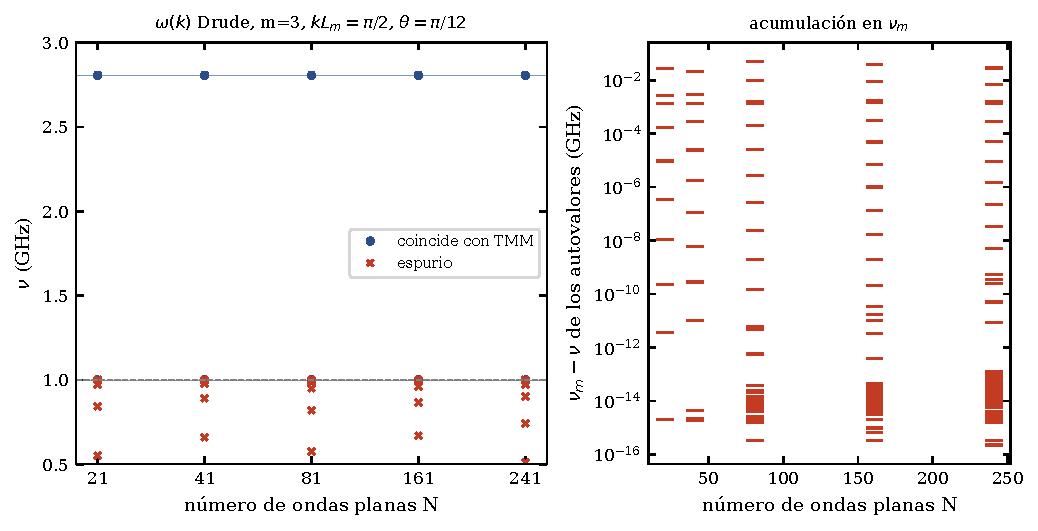
\includegraphics[width=\linewidth]{pwe/spectral_pollution/output/spectral_pollution.pdf}
    \end{column}
    \begin{column}{0.40\textwidth}
      \footnotesize
      $m=3$, $\theta=\pi/12$, $kL_m=\pi/2$, $N=21\dots241$:
      \begin{itemize}
        \item La TMM da \textbf{dos} frecuencias en 0.5--3~GHz: 0.99852 y 2.80589~GHz (azul).
        \item El QEP las contiene, pero añade autovalores \textbf{espurios} (rojo) que no convergen con $N$.
        \item Se acumulan en $\num$, a distancias de $10^{-2}$ a $10^{-16}$~GHz.
      \end{itemize}
      \begin{alertblock}{Conclusión}
        Distinguir los autovalores físicos exigiría comprobar cada uno con la TMM: la forma $\omega(k)$ no sirve aquí.
      \end{alertblock}
    \end{column}
  \end{columns}
\end{frame}

% =====================================================================
\section{La solución: $k(\omega)$ con la regla inversa}
% =====================================================================

\begin{frame}{Idea clave: invertir los papeles de $\omega$ y $k$}
  \centering
  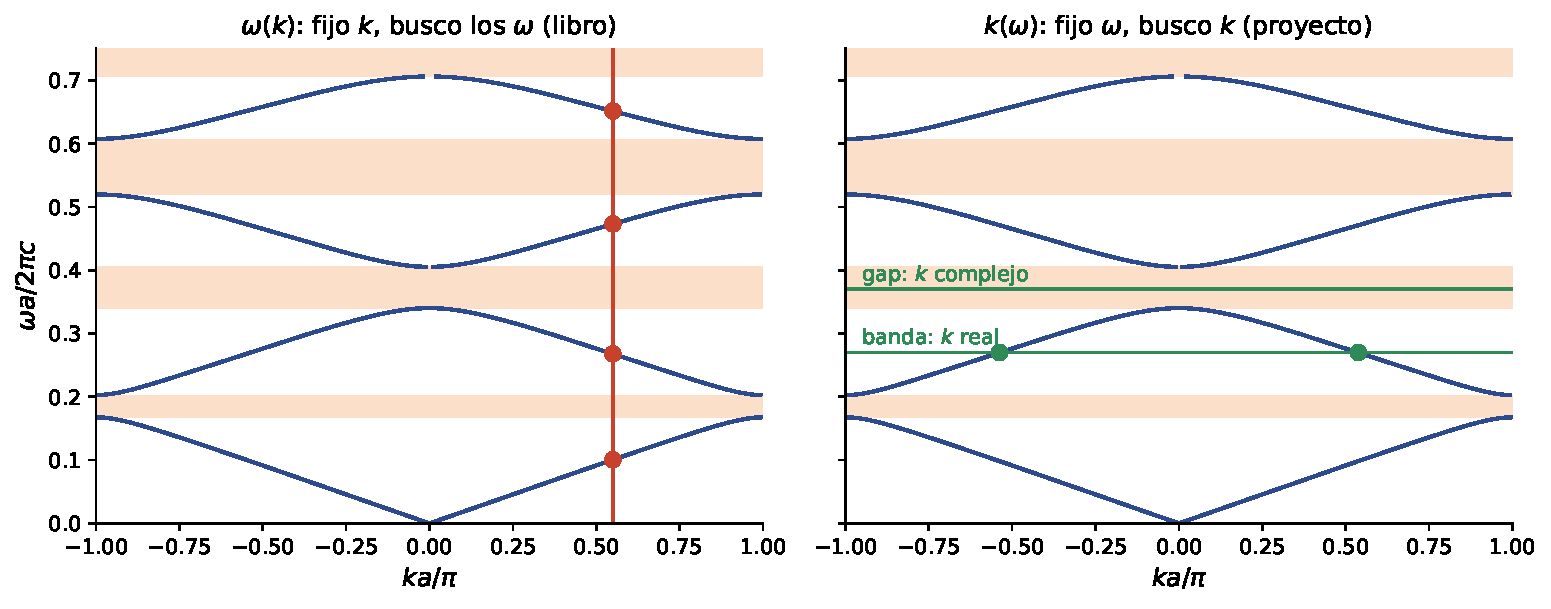
\includegraphics[width=\linewidth,height=0.55\textheight,keepaspectratio]{omega_k_vs_k_omega.pdf}
  \raggedright\small
  \begin{columns}[T]
    \begin{column}{0.48\textwidth}
      \textbf{$\omega(k)$}: fijo $k$, los autovalores son frecuencias. Con Drude, $\varepsilon(\omega)$ y $\mu(\omega)$
      están dentro de la matriz: problema no lineal.
    \end{column}
    \begin{column}{0.48\textwidth}
      \textbf{$k(\omega)$}: fijo $\omega$ (lo que barren todas las figuras del paper); $\varepsilon_B$ y
      $\mu_B$ son \textbf{números}. En un gap, $k$ es complejo y eso también es información.
    \end{column}
  \end{columns}
\end{frame}

\begin{frame}{Reglas de factorización de Li}
  \begin{columns}[c]
    \begin{column}{0.55\textwidth}
      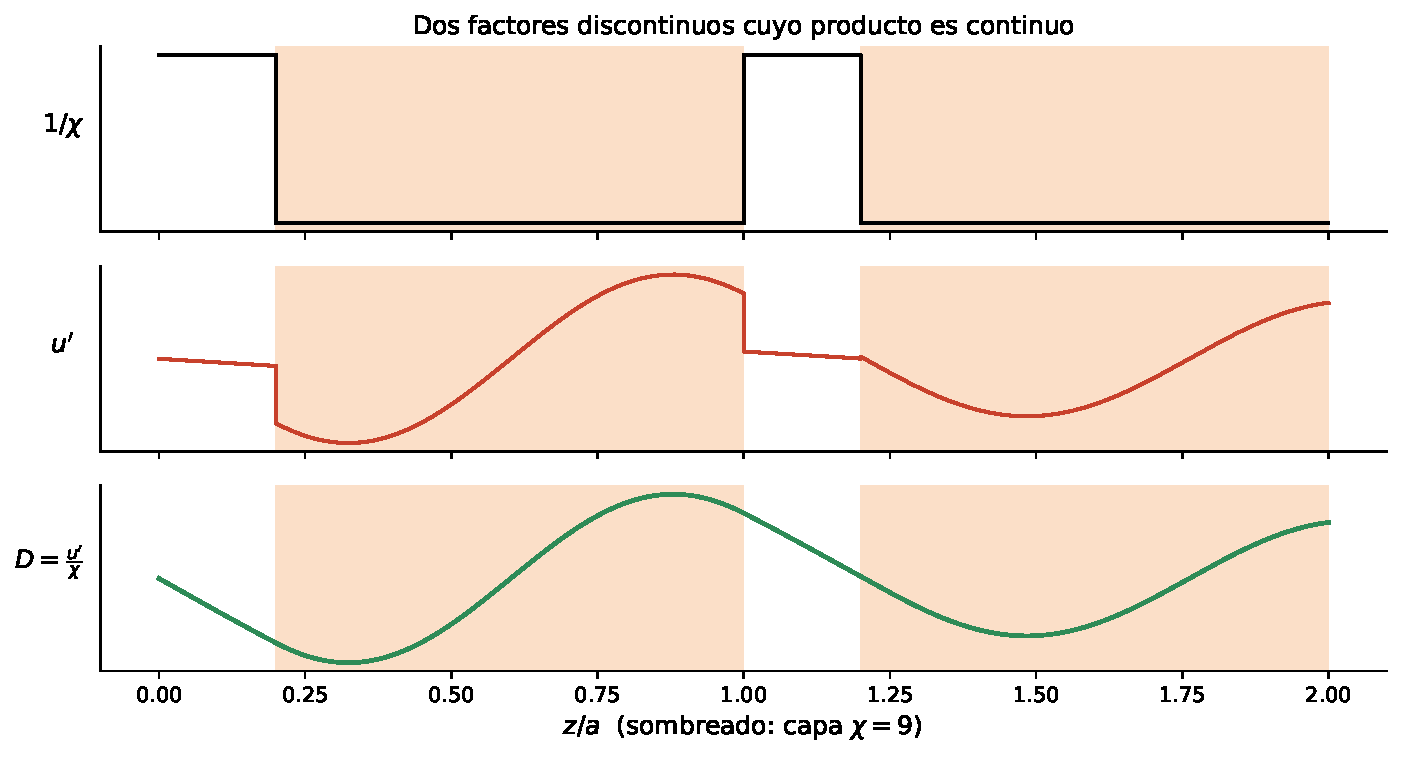
\includegraphics[width=\linewidth]{regla_li.pdf}
    \end{column}
    \begin{column}{0.43\textwidth}
      \footnotesize
      El flujo $D=\frac1\chi u'$ es producto de dos funciones que saltan en las interfaces, pero $D$ es continuo.
      Li (1996) demostró:
      \begin{itemize}
        \item \textbf{Laurent}: $[D]\approx\toep{1/\chi}[u']$ converge lento y a un valor incorrecto.
        \item \textbf{Inversa}: de $[u']=\toep{\chi}[D]$ se despeja
          \[[D]\approx\toep{\chi}^{-1}[u'],\]
          que solo desarrolla productos con un factor continuo.
      \end{itemize}
      \begin{exampleblock}{En el proyecto}
        $P=\toep{\chi}^{-1}$ (\texttt{rule="inverse"}). Con Drude, $m=3$, $N=97$: error en $R$ de
        $6\times10^{-7}$ frente a $1.8\times10^{-2}$ (TE) y $0.17$ (TM) con Laurent.
      \end{exampleblock}
    \end{column}
  \end{columns}
\end{frame}

\begin{frame}{El problema cuadrático en $k$}
  \small
  Adimensionalizamos con el período: $\kt=kL_m$, $\tilde G=\mathrm{diag}(2\pi n)$, $\tilde\kappa=\omega L_m/c$,
  $\tilde q=qL_m$. Con $K=\kt I+\tilde G$ la ecuación maestra queda
  \begin{block}{QEP en $\kt$ (fijo $\omega$)}
    \[\kt^{\,2}P+\kt\,(P\tilde G+\tilde GP)+(\tilde GP\tilde G-F)=0,\qquad
      F=\tilde\kappa^2\toep{\psi}-\tilde q^{\,2}\toep{1/\chi}\]
  \end{block}
  \begin{columns}[T]
    \begin{column}{0.52\textwidth}
      Con $\mathbf x=(\mathbf u,\kt\mathbf u)$ se linealiza en forma \textbf{compañera}:
      \[\begin{pmatrix}0&I\\-P^{-1}A_0&-P^{-1}A_1\end{pmatrix}\mathbf x=\kt\,\mathbf x,\]
      con $A_1=P\tilde G+\tilde GP$ y $A_0=\tilde GP\tilde G-F$.
    \end{column}
    \begin{column}{0.45\textwidth}
      \begin{exampleblock}{Ventaja de la regla inversa}
        $P^{-1}=\toep{\chi}$: la matriz compañera se arma \textbf{sin invertir nada}. Un solo
        \texttt{numpy.linalg.eigvals} de tamaño $2N\times2N$ por frecuencia.
      \end{exampleblock}
    \end{column}
  \end{columns}
\end{frame}

\begin{frame}{Seleccionar el modo físico y obtener $R$}
  \centering
  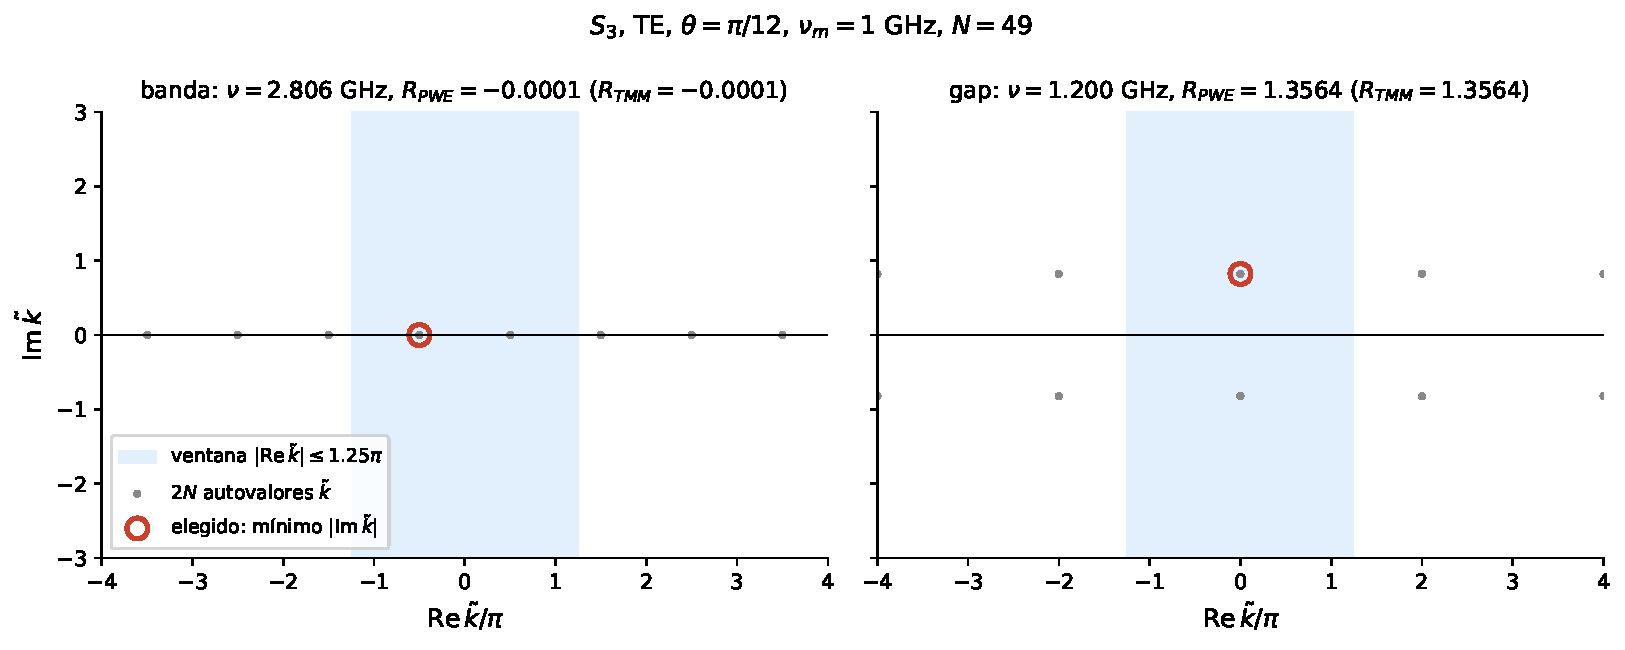
\includegraphics[width=\linewidth,height=0.50\textheight,keepaspectratio]{plano_k_complejo.pdf}
  \raggedright\small
  \begin{columns}[T]
    \begin{column}{0.50\textwidth}
      Los $2N$ autovalores incluyen cada modo con sus copias $\pm\kt+2\pi j$. Se elige, dentro de
      $|\mathrm{Re}\,\kt|\le1.25\pi$, el de \textbf{menor} $|\mathrm{Im}\,\kt|$ (el que menos decae):
      \[R_{\rm PWE}(\omega)=\mathrm{Re}\cos\kt .\]
    \end{column}
    \begin{column}{0.46\textwidth}
      \begin{itemize}
        \item Banda: $\kt$ real, $|R|\le1$.
        \item Gap: $\kt=j\pi+i\gamma$, $R=\pm\cosh\gamma$, $|R|>1$.
      \end{itemize}
      El PWE entrega la misma $R$ que la TMM y se compara punto a punto.
    \end{column}
  \end{columns}
\end{frame}

\begin{frame}{Convergencia en la superred de Drude}
  \begin{columns}[c]
    \begin{column}{0.58\textwidth}
      \figfull{pwe/convergence/output/drude_convergence.pdf}
    \end{column}
    \begin{column}{0.40\textwidth}
      \small
      Parámetros de la Fig.~5 del paper, $\theta=\pi/6$, 60 frecuencias entre 0.3 y 5~GHz; error máximo en $R$
      dentro de las bandas frente a la TMM.
      \begin{itemize}
        \item \textbf{Inversa} (continua): $\sim N^{-3}$ para $m=3,4,5$, en TE y TM.
        \item \textbf{Laurent} (trazos): se estanca en $10^{-2}$--$1$; en TM llega a $10^{2}$, porque allí
          $\varepsilon_B$, que está dentro de la derivada, cambia de signo.
      \end{itemize}
    \end{column}
  \end{columns}
\end{frame}

\begin{frame}{Límite de validez junto a $\num$}
  \begin{columns}[c]
    \begin{column}{0.58\textwidth}
      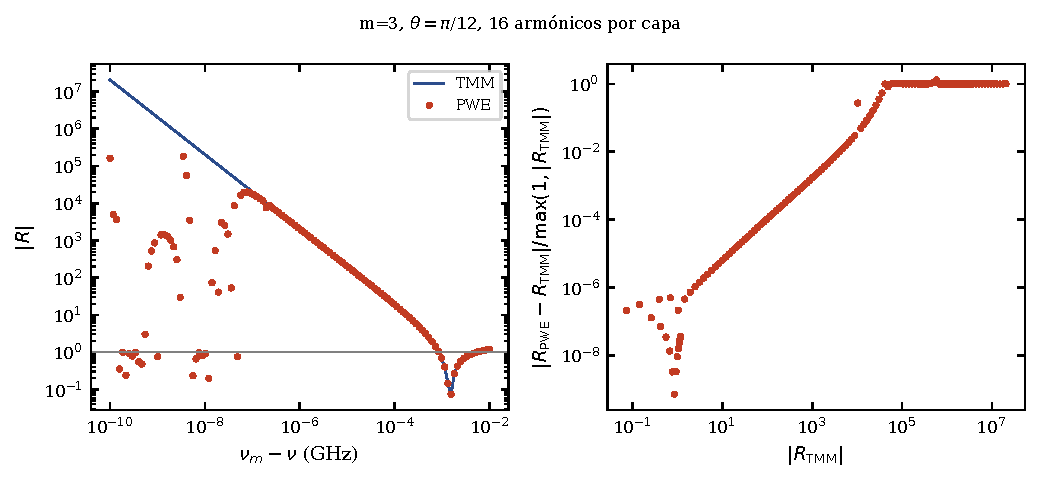
\includegraphics[width=\linewidth]{pwe/convergence/output/validity_near_nu_m.pdf}
    \end{column}
    \begin{column}{0.40\textwidth}
      \small
      Justo debajo de $\num$, $\mu_B\to0^-$ y la onda es muy evanescente en las capas B: $|R|$ llega a $10^4$
      y más. El modo está amortiguado exponencialmente y el truncamiento de Fourier no lo representa.
      \begin{alertblock}{Salvaguardas en el código}
        \begin{enumerate}
          \item Las mallas del PWE terminan a $10^{-7}$~GHz de $\num$.
          \item Cada banda se \textbf{revalida} con $1.5N$ ondas planas: se acepta si
            $|R_{1.5N}|\le1$ y $|R_N-R_{1.5N}|\le10^{-2}$.
        \end{enumerate}
      \end{alertblock}
    \end{column}
  \end{columns}
\end{frame}

% =====================================================================
\section{Implementación computacional}
% =====================================================================

\begin{frame}{Arquitectura del PWE en el paquete}
  \centering
  \begin{tikzpicture}[
      mod/.style={rounded corners=3pt,draw=fondo,fill=celeste!55,line width=0.7pt,
                  minimum height=0.95cm,minimum width=2.6cm,align=center,font=\scriptsize},
      io/.style={mod,fill=naranja!45},
      fl/.style={-{Stealth[length=2.5mm]},line width=1pt,fondo},
      node distance=0.5cm and 0.6cm]
    \node[io] (yaml) {\texttt{configs/pwe/*.yaml}\\$h$, regla, malla};
    \node[mod,right=of yaml] (cfg) {\texttt{config/}\\Pydantic};
    \node[mod,right=of cfg] (solver) {\texttt{PWESolver}\\\texttt{solver.py}};
    \node[mod,right=of solver] (bloch) {\texttt{solve\_bloch}\\\texttt{bloch.py}};
    \node[mod,below=0.9cm of bloch] (four) {\texttt{fourier.py}\\\texttt{CellFourier}, $\toep{f}$};
    \node[mod,left=of four] (qep) {\texttt{qep\_matrices}\\compañera + \texttt{eigvals}};
    \node[mod,left=of qep] (sel) {\texttt{select\_bloch\_}\\\texttt{wavevector}: $R$};
    \node[mod,left=of sel] (scan) {\texttt{DispersionScan}\\\texttt{solvers/scan.py}};
    \node[mod,below=0.9cm of scan] (edges) {\texttt{analysis/}\\bordes, Brent, validación};
    \node[mod,right=of edges] (repro) {\texttt{reproduction/}\\Figs.~1--6};
    \node[io,right=of repro] (out) {\texttt{results/pwe/}\\PDF, PNG, JSON};
    \node[mod,right=of out] (cmp) {\texttt{benchmark/}\\TMM vs PWE};
    \draw[fl] (yaml) -- (cfg);
    \draw[fl] (cfg) -- (solver);
    \draw[fl] (solver) -- (bloch);
    \draw[fl] (bloch) -- (four);
    \draw[fl] (four) -- (qep);
    \draw[fl] (qep) -- (sel);
    \draw[fl] (sel) -- (scan);
    \draw[fl] (scan) -- (edges);
    \draw[fl] (edges) -- (repro);
    \draw[fl] (repro) -- (out);
    \draw[fl] (out) -- (cmp);
    \node[draw=rojo,dashed,rounded corners,fit=(bloch)(four)(qep)(sel),inner sep=5pt,
          label={[font=\scriptsize,rojo]above:por frecuencia, repartido en procesos}] {};
  \end{tikzpicture}
  \vspace{0.3em}

  \small Todo en \texttt{src/fibonacci\_photonics/solvers/pwe/}, independiente de \texttt{solvers/tmm/}. Del
  \texttt{DispersionScan} en adelante, TMM y PWE comparten el mismo código.
\end{frame}

\begin{frame}[fragile]{Un contrato común para los dos métodos}
  \begin{columns}[T]
    \begin{column}{0.52\textwidth}
\begin{lstlisting}
from fibonacci_photonics import (
    PWESolver, TMMSolver, load_spec)

spec = load_spec("figure_03.yaml")
nu = np.linspace(0.5, 3.0, 2000)          # GHz

tmm = TMMSolver(spec)
pwe = PWESolver(spec, harmonics_per_layer=8,
                rule="inverse", workers=8)

for solver in (tmm, pwe):
    scan = solver.scan(m=4, theta=np.pi / 12,
                       nu_ghz=nu, polarization="TE")
    print(solver.method, scan.allowed.mean())
\end{lstlisting}
    \end{column}
    \begin{column}{0.46\textwidth}
      \small
      \begin{itemize}
        \item \texttt{DispersionSolver} (Protocol): \texttt{semitrace}, \texttt{scan} y \texttt{evaluator}
          con las mismas firmas y unidades (GHz, rad).
        \item Las funciones de análisis reciben \emph{cualquier} solver: bordes, subbandas y comparación no saben de
          dónde viene $R$.
        \item Validación de entradas común: frecuencias finitas y $>0$, $\theta\in[0,\pi/2]$, orden $m$ entero.
        \item \texttt{convergence\_report} compara con $1.5N$ ondas planas y emite \texttt{ConvergenceWarning} si no
          converge.
      \end{itemize}
    \end{column}
  \end{columns}
\end{frame}

\begin{frame}[fragile]{El núcleo del solver $k(\omega)$}
  \begin{columns}[T]
    \begin{column}{0.58\textwidth}
\begin{lstlisting}
# solvers/pwe/bloch.py  (una frecuencia omega)
t_chi = cell.toeplitz(chi_a, chi_b)          # [[χ]]
t_inv_chi = cell.toeplitz(1/chi_a, 1/chi_b)  # [[1/χ]]
p = np.linalg.inv(t_chi)                     # regla inversa
f = kappa**2 * cell.toeplitz(psi_a, psi_b) - q2 * t_inv_chi
a1 = p @ g + g @ p
a0 = g @ p @ g - f

companion = np.zeros((2*N, 2*N), complex)
companion[:N, N:] = np.eye(N)
companion[N:, :N] = -t_chi @ a0              # P^-1 = [[χ]]
companion[N:, N:] = -t_chi @ a1
k = np.linalg.eigvals(companion)             # 2N autovalores

inside = k[np.abs(k.real) <= 1.25 * np.pi]
k_phys = inside[np.argmin(np.abs(inside.imag))]
r = np.cos(k_phys).real                      # R_PWE
\end{lstlisting}
    \end{column}
    \begin{column}{0.40\textwidth}
      \small
      \begin{itemize}
        \item \texttt{chi, psi} según la polarización: en TE, $\chi=\mu$ y $\psi=\varepsilon$.
        \item \texttt{g} $=\mathrm{diag}(2\pi n)$; \texttt{kappa} $=\omega L_m/c$; \texttt{q2} $=\tilde q^2$.
        \item Costo: un \texttt{eigvals} de $2N\times2N$, es decir $O(N^3)$ por frecuencia.
        \item Las frecuencias son independientes: \texttt{solve\_bloch} las reparte en bloques entre procesos, con
          un hilo de BLAS en cada uno.
        \item En los polos de Drude el problema es singular y $R$ queda en \texttt{NaN}.
      \end{itemize}
    \end{column}
  \end{columns}
\end{frame}

\begin{frame}{Del barrido a las subbandas: localización y validación}
  \begin{columns}[T]
    \begin{column}{0.52\textwidth}
      \small
      Las subbandas de las Figs.~5--6 miden de $6\times10^{-8}$ a $4\times10^{-2}$~GHz y están pegadas a
      $\num$. TMM y PWE usan el \textbf{mismo} localizador (\texttt{analysis/band\_edges.py}):
      \begin{enumerate}
        \item Malla logarítmica en $\num-\nu$ (\texttt{plasmon\_grid}).
        \item Cambios de signo de $|R|-1$ (bordes) y de $R$ (bandas completas entre dos muestras).
        \item Refinamiento de cada borde con el método de \textbf{Brent} sobre el evaluador escalar de $R$.
        \item Solo PWE: \texttt{validate\_bands} con $1.5N$ ondas planas.
      \end{enumerate}
    \end{column}
    \begin{column}{0.46\textwidth}
      \begin{block}{Parámetros numéricos (\texttt{configs/pwe/})}
        \footnotesize
        \begin{tabular}{llc}
          \toprule
          Figura & $h$ & frecuencias \\
          \midrule
          1, 3 & 8 & 1500 \\
          2 & 8 & 3000 \\
          4 & 16 & 4000 \\
          5, 6 ($m\le4$) & 16 & 300 (log.) \\
          5, 6 ($m=5,6$) & 8 & 300 (log.) \\
          \bottomrule
        \end{tabular}
      \end{block}
      \small La física (espesores, $\nue$, $\num$, ángulos) se lee de los mismos
      \texttt{configs/figure\_0N.yaml} que usa la TMM; todos se validan con Pydantic.
    \end{column}
  \end{columns}
\end{frame}

\begin{frame}{Pruebas automáticas del PWE}
  \begin{columns}[T]
    \begin{column}{0.50\textwidth}
      \begin{block}{Casos analíticos (\texttt{tests/analytic/})}
        \small
        \begin{itemize}
          \item Límite homogéneo: $R=\cos(\kappa nL)$, sin gaps, con TMM y PWE.
          \item Bicapa de cuarto de onda: $R=-5/3$ en el centro del gap y $R=1$ a media onda; el PWE la
            reproduce a $10^{-4}$.
          \item TE = TM a $\theta=0$ y dualidad $\varepsilon\leftrightarrow\mu$.
          \item Parseval para los coeficientes de las indicadoras de la celda.
        \end{itemize}
      \end{block}
    \end{column}
    \begin{column}{0.48\textwidth}
      \begin{block}{Unitarias y de regresión}
        \small
        \begin{itemize}
          \item Fourier: ec.~(4.38) del libro, $[\![f]\!]$ hermítica, síntesis convergente.
          \item Bandas del libro y $R$ de Drude frente a la TMM; la regla inversa converge más rápido que Laurent.
          \item Selección del modo que se propaga; paralelo = serie; contaminación de $\omega(k)$.
          \item Contrato común (entradas inválidas, \texttt{ConvergenceWarning}), conteo $F_{m-2}$ y
            \texttt{reference\_values.json}.
        \end{itemize}
      \end{block}
      \small \texttt{make tests} y \texttt{make lint} (ruff + mypy).
    \end{column}
  \end{columns}
\end{frame}

% =====================================================================
\section{Resultados}
% =====================================================================

\begin{frame}{Figura 1 con ondas planas ($\nue=\num=3$ GHz)}
  \begin{columns}[c]
    \begin{column}{0.62\textwidth}
      \figfull{pwe/figure_01/output/figure_01.pdf}
    \end{column}
    \begin{column}{0.36\textwidth}
      \small
      TE, $m=3,4$, cuatro ángulos; $h=8$ armónicos por capa.
      \begin{itemize}
        \item Gap de índice medio nulo y banda plasmón-polaritón junto a $\num$ en incidencia oblicua.
        \item Error máximo en $R$ frente a la TMM: $\sim\!2\times10^{-2}$, en el extremo de 0.15~GHz, donde
          $\varepsilon_B=\mu_B\approx-399$.
        \item Clasificación banda/gap idéntica en más del 99.9\,\% de las frecuencias.
      \end{itemize}
    \end{column}
  \end{columns}
\end{frame}

\begin{frame}{Superposición TMM--PWE: Figuras 1 y 3}
  \begin{columns}[c]
    \begin{column}{0.49\textwidth}
      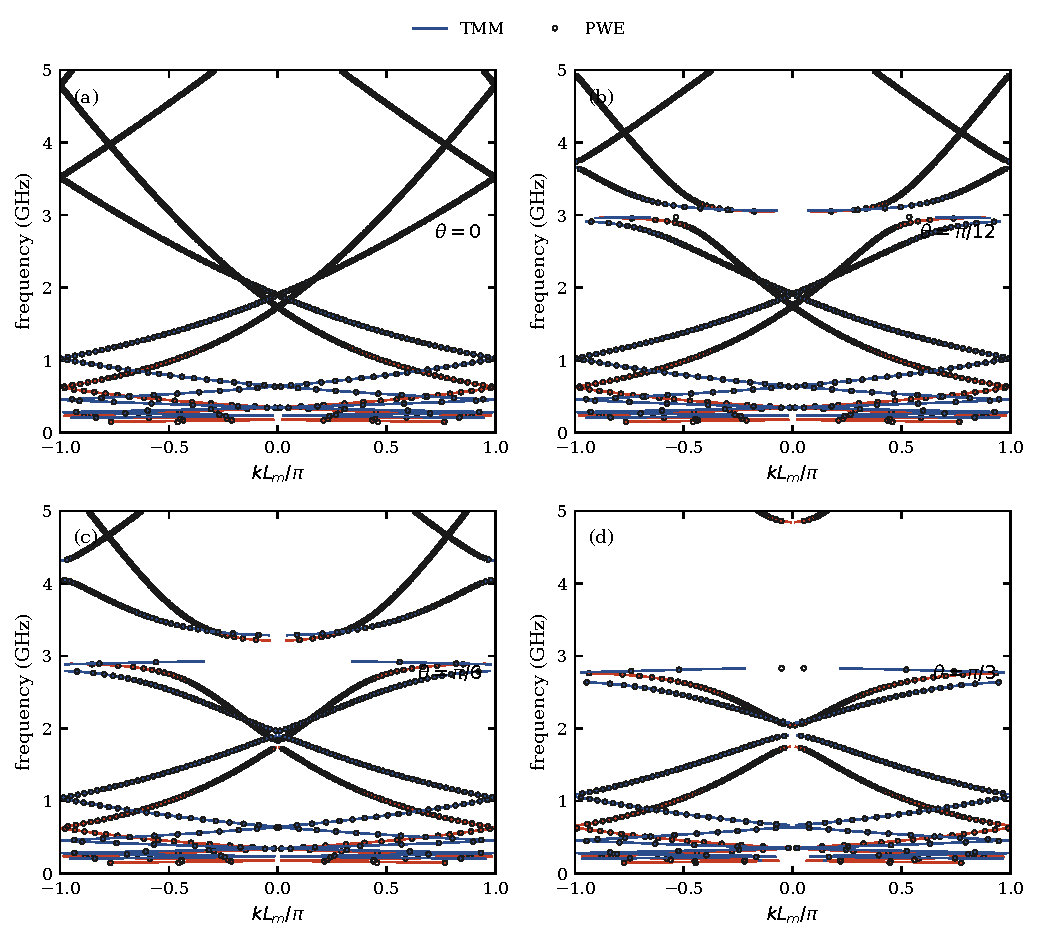
\includegraphics[width=\linewidth,height=0.72\textheight,keepaspectratio]{comparison/figure_01/output/figure_01_overlay.pdf}
    \end{column}
    \begin{column}{0.49\textwidth}
      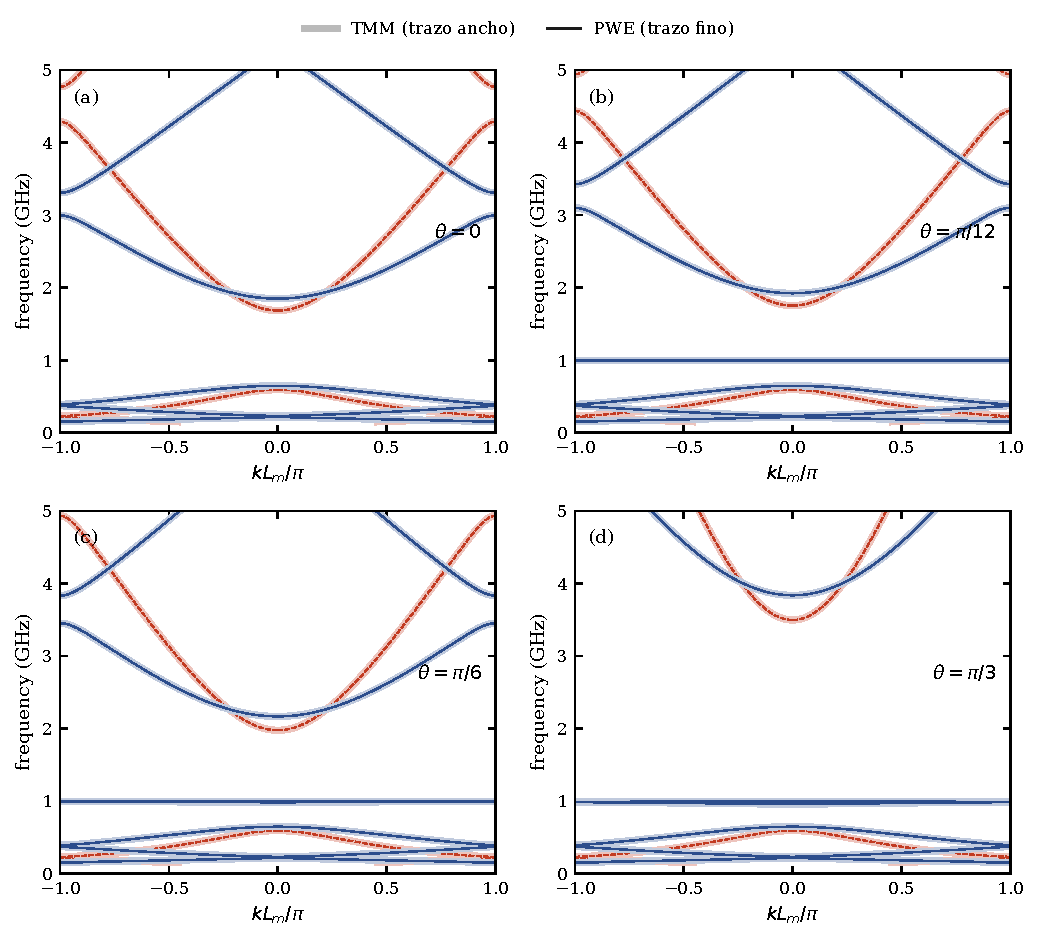
\includegraphics[width=\linewidth,height=0.72\textheight,keepaspectratio]{comparison/figure_03/output/figure_03_overlay.pdf}
    \end{column}
  \end{columns}
  \small Líneas: TMM; puntos: PWE. Error máximo en $R$ dentro de las bandas: $2\times10^{-2}$ (Fig.~1),
  $4.5\times10^{-4}$ (Fig.~3).
\end{frame}

\begin{frame}{Figuras 2 y 4: contar las subbandas}
  \begin{columns}[c]
    \begin{column}{0.58\textwidth}
      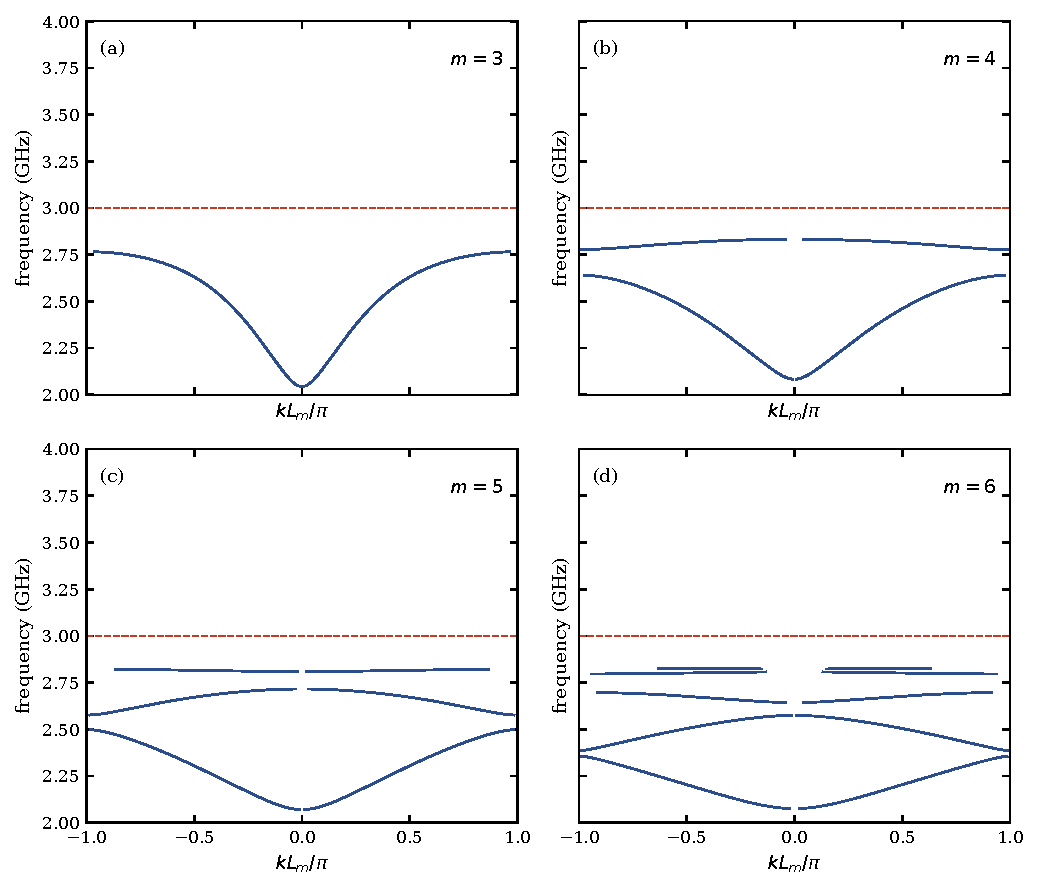
\includegraphics[width=\linewidth,height=0.40\textheight,keepaspectratio]{pwe/figure_02/output/figure_02.pdf}\\
      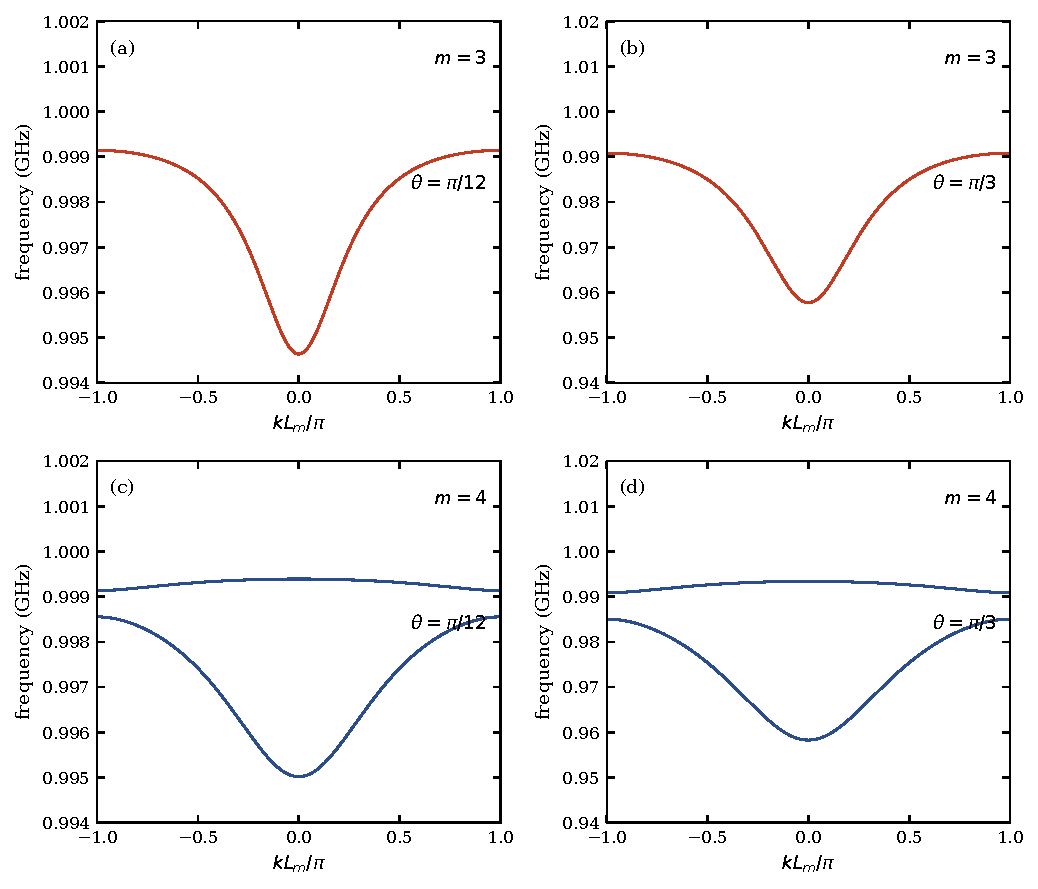
\includegraphics[width=\linewidth,height=0.40\textheight,keepaspectratio]{pwe/figure_04/output/figure_04.pdf}
    \end{column}
    \begin{column}{0.40\textwidth}
      \footnotesize
      \IfFileExists{../results/comparison/tables/mode_counts.tex}
        {\resizebox{\linewidth}{!}{\begin{tabular}{rrrrrr}
\toprule
Fig. & $m$ & ángulo & $F_{m-2}$ & TMM & PWE \\
\midrule
2 & 3 & $\theta=\pi/3$ & 1 & 1 & 1 \\
2 & 4 & $\theta=\pi/3$ & 2 & 2 & 2 \\
2 & 5 & $\theta=\pi/3$ & 3 & 3 & 3 \\
2 & 6 & $\theta=\pi/3$ & 5 & 5 & 5 \\
4 & 3 & $\theta=\pi/12$ & 1 & 1 & 1 \\
4 & 3 & $\theta=\pi/3$ & 1 & 1 & 1 \\
4 & 4 & $\theta=\pi/12$ & 2 & 2 & 2 \\
4 & 4 & $\theta=\pi/3$ & 2 & 2 & 2 \\
\bottomrule
\end{tabular}
}}{}
      \begin{exampleblock}{Resultado}
        \small PWE y TMM encuentran exactamente $F_{m-2}=1,2,3,5$ subbandas.
      \end{exampleblock}
    \end{column}
  \end{columns}
\end{frame}

\begin{frame}{Figuras 5 y 6: bordes de subbandas frente al orden y al ángulo}
  \begin{columns}[c]
    \begin{column}{0.49\textwidth}
      \figfull{pwe/figure_05/output/figure_05.pdf}
    \end{column}
    \begin{column}{0.49\textwidth}
      \footnotesize
      \centering
      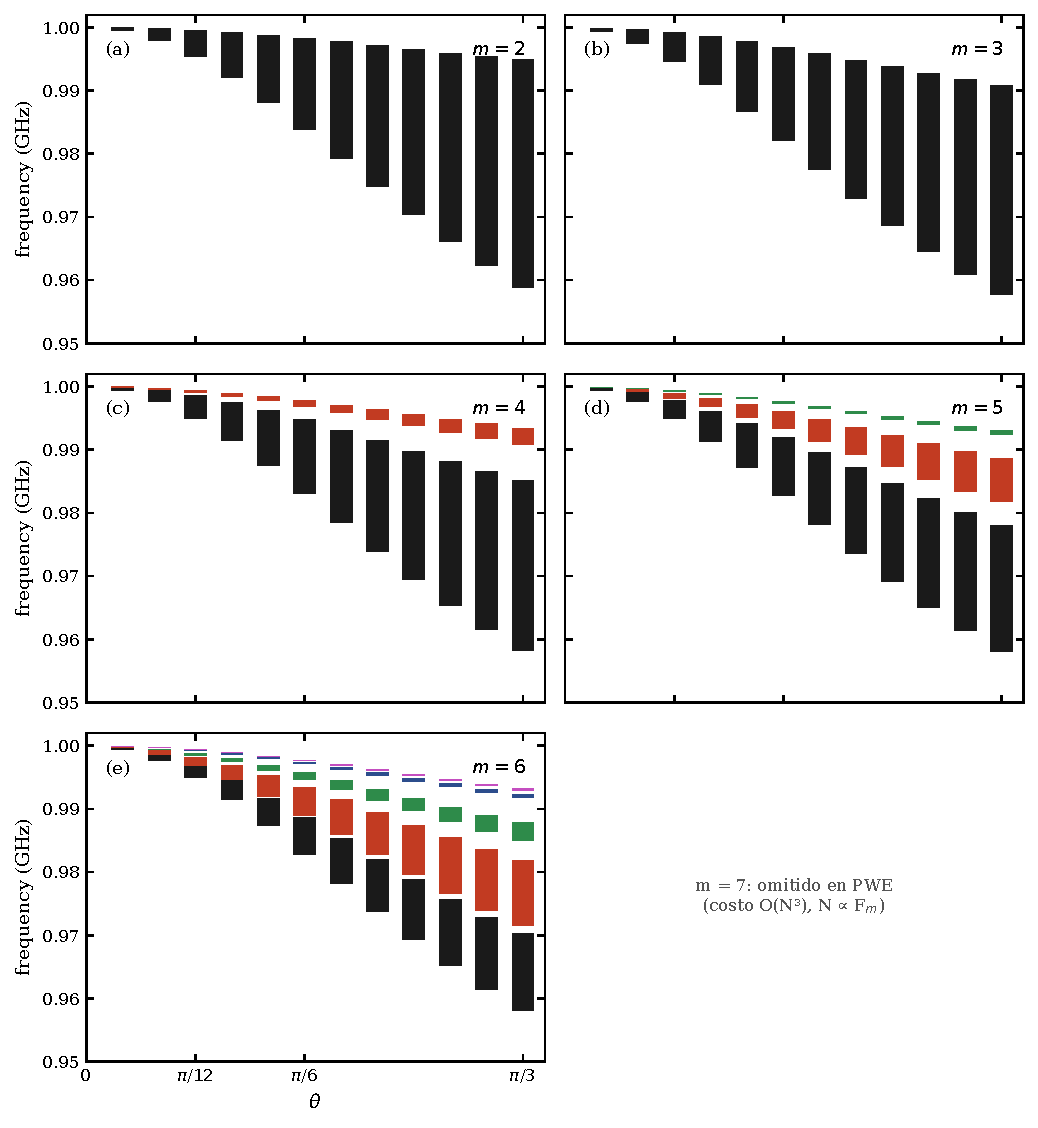
\includegraphics[width=\linewidth,height=0.38\textheight,keepaspectratio]{pwe/figure_06/output/figure_06.pdf}
      \raggedright
      \begin{itemize}
        \item $m=2\dots6$ ($m=7,8$ solo con TMM, por costo); con el PWE se omite $\theta=0$, donde las
          subbandas quedan a menos de $10^{-5}$~GHz de $\num$.
        \item 70 casos comparados: error de borde $\le10^{-7}$~GHz y error relativo de ancho $\le4\times10^{-6}$.
      \end{itemize}
    \end{column}
  \end{columns}
\end{frame}

\begin{frame}{Costo: por qué la TMM sigue siendo el método de producción}
  \begin{columns}[c]
    \begin{column}{0.55\textwidth}
      \figfull{pwe/convergence/output/cost_and_accuracy.pdf}
    \end{column}
    \begin{column}{0.43\textwidth}
      \small
      \begin{itemize}
        \item PWE: $O(N^3)$ por frecuencia con $N=2hF_m+1$ y $F_m\sim\phi^m$: el costo crece como $\phi^{3m}$.
        \item Medido en un núcleo: el tiempo crece como $N^{\EffAlphaShort}$ (\EffPweLast{} por frecuencia con
          $m=\EffPweLastM$).
        \item TMM por recurrencia: $\sim\!\EffTmmRecMax~\mu$s por frecuencia hasta $m=\EffTmmMaxM$.
      \end{itemize}
      \begin{alertblock}{Las seis figuras del paper}
        TMM: \EffFigTmmTotal{}\qquad PWE: $\approx$\EffFigPweTotal{}
      \end{alertblock}
    \end{column}
  \end{columns}
\end{frame}

% =====================================================================
\section{Cierre}
% =====================================================================

\begin{frame}{Conclusiones}
  \begin{enumerate}
    \item El PWE del libro se extendió a la celda de Fibonacci con coeficientes de Fourier en forma cerrada y
      reproduce el capítulo 1D: bandas, síntesis, campo y bandas fuera del eje con Brewster.
    \item La forma $\omega(k)$ \textbf{falla} con metamateriales de Drude: problema cuadrático en $\omega^2$ y
      contaminación espectral acumulada en $\num$.
    \item La forma $k(\omega)$ con la \textbf{regla inversa de Li} resuelve el problema: da la misma semitraza que
      la TMM, el mismo conteo $F_{m-2}$ y bordes con errores relativos $<10^{-5}$.
    \item La regla de factorización es esencial: Laurent se estanca en $10^{-2}$--$1$; la inversa converge como
      $N^{-3}$.
    \item La TMM es el método óptimo en 1D; el PWE queda como verificación independiente y como base para
      cristales 2D.
  \end{enumerate}
\end{frame}

\begin{frame}{¿Cuándo usar cada método?}
  \centering
  \small
  \begin{tabular}{lll}
    \toprule
    & TMM & PWE ($k(\omega)$, regla inversa) \\
    \midrule
    Formulación & producto de matrices $2\times2$ & autovalores de una matriz $2N\times2N$ \\
    Exactitud en 1D & exacta (redondeo de máquina) & error $\propto N^{-3}$ \\
    Costo por frecuencia & $O(m)$, microsegundos & $O(N^3)$, de ms a decenas de s \\
    Junto a $\num$ & estable & falla en gaps profundos ($<10^{-6}$ GHz) \\
    Dispersión de Drude & trivial & obliga a la forma $k(\omega)$ \\
    Generaliza a 2D/3D & no & sí \\
    Papel en el proyecto & producción & verificación independiente \\
    \bottomrule
  \end{tabular}
\end{frame}

\begin{frame}[fragile]{Cómo reproducir los resultados del PWE}
\footnotesize
\begin{verbatim}
pip install -r requirements.txt && pip install -e .

python scripts/run_figure.py 3 --method pwe          # una figura con el PWE
python scripts/run_figure.py all --method both        # las seis, TMM y PWE
python scripts/pwe/run_all.py                         # PWE + estudios (PWE_WORKERS=n)
python scripts/comparison/run_all.py                  # superposiciones y tablas TMM vs PWE
make presentation-pwe                                 # esta presentación
\end{verbatim}
  \vspace{0.3em}
  \small
  \begin{itemize}
    \item Parámetros numéricos: \texttt{configs/pwe/figure\_0N.yaml} (armónicos por capa $h$, regla, malla).
    \item Salidas: \texttt{results/pwe/} y \texttt{results/comparison/}.
    \item Documento completo: \texttt{docs/metodo\_ondas\_planas/metodo\_ondas\_planas.pdf} y el anexo
      \texttt{comparacion\_tmm\_pwe.pdf}.
  \end{itemize}
\end{frame}

\begin{frame}{Referencias}
  \small
  \begin{itemize}
    \item E.~Reyes-Gómez \textit{et al.}, ``Plasmon polaritons in photonic metamaterial Fibonacci superlattices'',
      Phys.\ Rev.\ B \textbf{81}, 153101 (2010).
    \item I.\,A.~Sukhoivanov e I.\,V.~Guryev, \textit{Photonic Crystals: Physics and Practical Modeling},
      Springer (2009), cap.~4.
    \item L.~Li, ``Use of Fourier series in the analysis of discontinuous periodic structures'',
      J.\ Opt.\ Soc.\ Am.\ A \textbf{13}, 1870 (1996).
    \item F.~Tisseur y K.~Meerbergen, ``The quadratic eigenvalue problem'', SIAM Review \textbf{43}, 235 (2001).
    \item A.~Tip, A.~Moroz y J.-M.~Combes, ``Band structure of absorptive photonic crystals'',
      J.\ Phys.\ A \textbf{33}, 6223 (2000).
    \item J.\,D.~Joannopoulos \textit{et al.}, \textit{Photonic Crystals: Molding the Flow of Light}, 2.ª ed.,
      Princeton (2008).
  \end{itemize}
\end{frame}

\begin{frame}[standout]
  ¡Gracias!\\[0.5em]
  {\small ¿Preguntas?}
\end{frame}

\end{document}
